\documentclass[11pt,a4paper]{scrartcl}
\usepackage[utf8]{inputenc}
\usepackage{amsmath}
\usepackage{amsfonts}
\usepackage{pgfpages}
\usepackage{amssymb}
\usepackage[hidelinks]{hyperref}
\usepackage[utf8]{inputenc}
\usepackage[ngerman]{babel}
\usepackage[autostyle]{csquotes}
\usepackage{eurosym}
\usepackage[left=2.54cm,right=2.54cm,top=2.54cm,bottom=2.54cm]{geometry}
\usepackage[affil-it]{authblk}

\author{Leonard Hackel, Jochen Jacobs, Niklas Schelten}
\affil{Herder-Gymnasium}
\title{Manual zur Benutzung des RF1000}
\begin{document}
\maketitle
\begin{center}
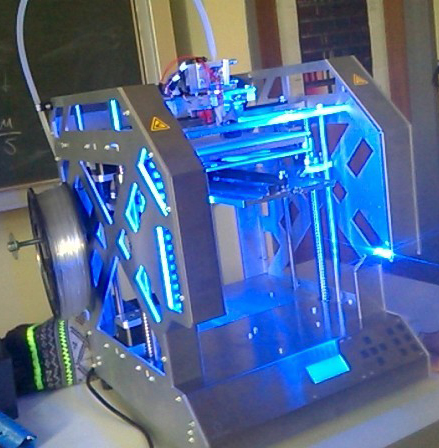
\includegraphics[scale=0.75]{res/31_1.jpg}
\end{center}
\pagebreak
\tableofcontents
\vspace{11pt}
%---------------------------Jochen----------------------------------------------
\section{Erstellen von 3D Objekten}
Für die Erstellung von 3D-Objekten ist die Verwendung von spezieller 3D-Software notwendig. Welche Software am sinnvollsten ist, hängt von dem zu erstellenden Objekt ab. Organische Objekte werden am Besten mit einem \enquote{normalen} 3D-Programm wie \textbf{Blender} erstellt, Während technische Objekte wie Zahnräder mit einem \textit{computer-aided design}-Programm (kurz CAD-Programm) erstellt - hier empfehle ich das kostenlose Programm \textbf{FreeCAD}. Beide Programme können Modelle als stl-Datei speichern - Dieses Format ist im 3D-Druck üblich. Im Gegensatz zur herkömmlichen 3D-Modellierung muss bei der Erstellung von zu druckenden Objekten nicht versucht werden die Anzahl der Polygone möglichst gering zu halten - im Gegenteil kann eine größere Anzahl an Polygonen nie schaden: Der 3D-Drucker beachtet die in der 3D-Graphik häufig benutzten Normalen nicht - dadurch erscheinen gedruckte Objekte sehr viel weniger Rund als sie auf dem Bildschirm aussehen.

Die Verwendung der beiden Programme ist sehr komplex und kann hier nicht komplett beschrieben werden. Besonders zu empfehlen sind gerade in diesem Bereich auch Tutorial-Videos auf YouTube. Als Beispiel zur Erstellung habe ich zu beiden Programmen je ein kurzes Video erstellt und auf YouTube hochgeladen:
\begin{itemize}
  \item \textbf{Blender} \url{https://youtu.be/BRPZsZmmzIY}
  \item \textbf{FreeCAD} \url{https://youtu.be/2ebwCnLCgOo}
\end{itemize}

\subsection*{Downloads:}
\addcontentsline{toc}{subsection}{Downloads}
\begin{itemize}
  \item \textbf{Blender} \url{http://www.blender.org/download/}
  \item \textbf{FreeCAD} \url{http://www.freecadweb.org/}
\end{itemize}

\subsection*{Andere M"oglichkeiten zur Generierung von 3D-Objekten}
\addcontentsline{toc}{subsection}{Andere M"oglichkeiten zur Generierung von 3D-Objekten}
3D-Objekte k"onnen auch erhalten werden, indem sie ...
\begin{itemize}
  \item[...] aus dem Internet heruntergeladen werden.
  \item[...] aus Hightmaps generiert werden (Hightmaps können direkt in Cura geladen werden)
  \item[...] aus Minecraft-Maps generiert werden (Cura $\rightarrow$ Tools $\rightarrow$ Minecraft Map Import)
  \item[...] mittel eines 3D-Scanners eingescanned werden
  \item[...] zufällig erstellt werden
\end{itemize}

%---------------------------Jochen----------------------------------------------
\section{Der Druck}
Für die folgende Erklärung benutzen wir die Drucker Software Cura (\url{https://software.ultimaker.com/}). Standardmäßig empfiehlt Conrad zwar eine modifizierte Variante des RepetierHost, die auf der SD-Karte beiliegt, aber wir empfehlen Cura zu benutzten, um mehr Einstellungsmöglichkeiten zu haben.
% neuen Drucker hinzufügen/vor der ersten Nutzung
\subsection*{Einen neuen Drucker hinzufügen}
\addcontentsline{toc}{subsection}{Einen neuen Drucker hinzufügen}
Da Cura den RF1000 nicht als Standard dabei hat, muss dieser vorher als neuer Drucker hinzugefügt werden. Dazu muss man unter \textit{Machine}, \textit{Add new machine...} dieser neu erstellt werden. Da er keine Voreinstellung ist, muss im \textit{Configuration Wizard} \textit{Other} gewählt werden, ebenso wie unter \textit{Other machine information} \textit{Custom...} ausgewählt sein muss. Nun kann man Namen (\textit{Machine name}), also RF1000, und Größe unter \textit{width}, \textit{depth} und \textit{height} einstellen (für den RF1000 245,235,200 mm in dieser Reihenfolge). \textit{Nozzle Size} ist standardmäßig 0.5 und für den RF1000 korrekt. Zusätzlich muss die Option \textit{Heated Bed} ausgewählt werden, die Option \textit{Bed center [...]} ist nicht zutreffend.\\
Danach müssen die anderen Einstellungen, welche sich auf der SD-Karte finden lassen, geladen werden. Dazu muss unter \textit{File}, \textit{Open Profile...} die Datei \textit{Settings.ini} geladen werden. Danach ist der RF1000 als Drucker eingestellt und kann für den Druck konfiguriert werden.\\
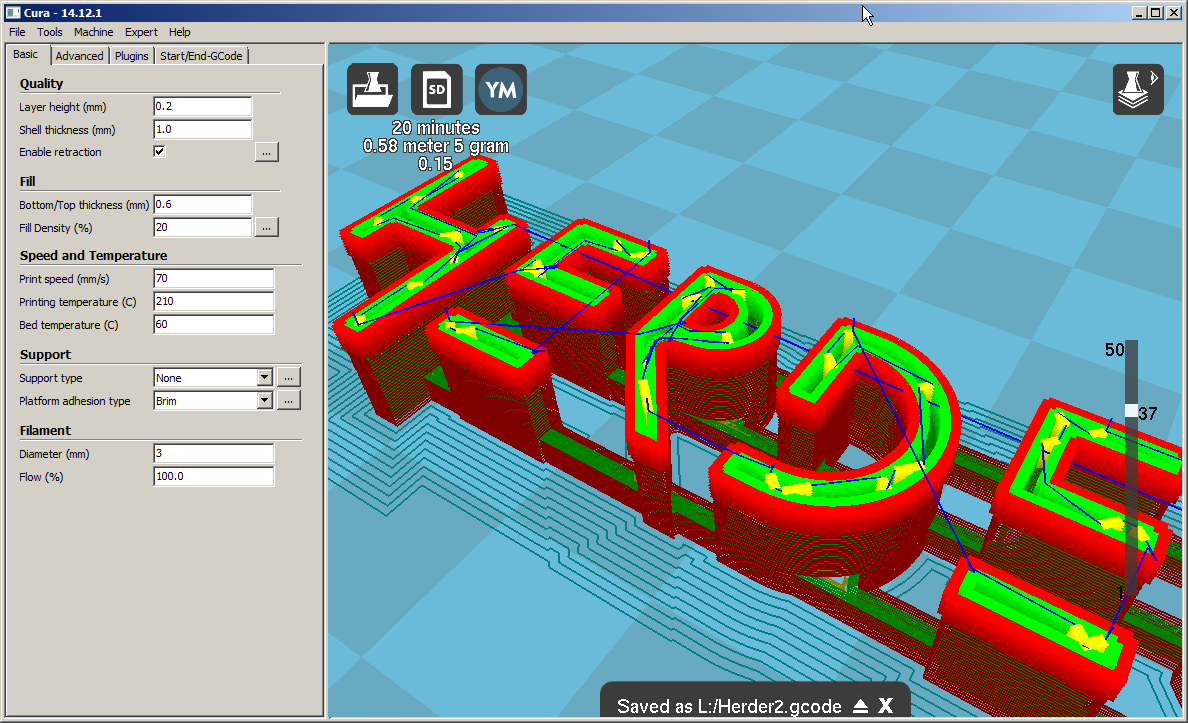
\includegraphics[scale=0.38]{res/Cura-window.png}\\

Um nun in diese Ansicht zu gelangen, muss man bei Cura im Reiter \textit{Expert} unter \textit{Switch to full settings} die Ansicht ändern. Dabei verschwinden die Schnelleinstellungen und diese Ansicht erscheint. Das hat den Vorteil, dass die Einstellungen viel genauer vorgenommen werden können.\\
\subsection*{Basic}
\addcontentsline{toc}{subsection}{Basic}
Das Vorschaufenster bei Cura besteht aus zwei großen Teilen. Auf der linken Seite sind die Einstellungen, auf der rechten ist eine 3D-Ansicht des Objektes. Dabei sind verschiedene Strecken in verschiedenen Farben angezeigt. Innenstrecken sind dabei grün, Druckstrecken, die später Außenflächen ergeben, sind rot, und Strecken, welche der Druckkopf zurücklegt, dabei aber nicht druckt, sind dünner und blau. In gelb dargestellt sind diejenigen Strecken, die später Füllung sind.\\
Die meisten Einstellungen sind selbsterklärend. So gibt die \textit{Layer heigt} an, wie hoch die einzelnen Drucklagen sind, wodurch damit auch die Anzahl der Lagen bestimmt wird. \textit{Shell thickness} gibt an, wie viele Spuren außen gedruckt werden, bevor der Bereich als Innenraum gilt und nur zu einem bestimmten Prozentsatz gefüllt wird. Dieser ist unter \textit{Fill Density} einstellbar. So wie \textit{Shell thickness} die Dicke der seitlichen Außenhaut angibt, gibt \textit{Bottom/Top thickness} dies für die oberen und unteren Schichten an.\\
\textit{Print speed} gibt an, wie schnell sich der Druckkopf relativ zu der Heizplatte bewegt, wenn er druckt (unter \textit{Advaced} gibt es noch andere Bewegungsarten). Hierbei gilt generell, dass eine geringere Geschwindigkeit die Qualität, allerdings auch die Druckzeit erhöht, wodurch ein geeignetes Mittelmaß zu finden ist. \textit{Printing temperature} und \textit{Bed temperature} sind von dem Druckmaterial abhängig, für PLA empfiehlt sich 210/60. Generell empfehlen wir die oben gezeigten Werte für die bisher genannten Einstellungen bei einem Druck mit PLA.\\
Unter \textit{Support} finden sich Einstellungen, die den Drucker bei schwereren Aufgaben wie Überhängen unterstützen. Sollte das Objekt Überhänge haben, empfehlen wir den \textit{Support type} \textit{Touching buildplate}, wenn es sich aber nur um kleine oder steile Überhänge handelt, ist ein Support nicht empfehlenswert (ab 60\% ist Support benötigt, ansonsten muss von Fall zu Fall unterschieden werden). Als \textit{Platform adhesion type} empfehlen wir einen \textit{Brim} der Breite 10, damit sich der Drucker \enquote{eindrucken} kann, wodurch Filamentaussetzer und Stotterer vermieden werden. Bei Objekten, welche leicht umfallen oder wackeln, ist ein \textit{Raft} zu empfehlen, da es den Druck stabilisiert. Allerdings kostet der Druck eines solchen viel Zeit.\\
\textit{Filament}-Settings sollten bei 3 (\textit{Diameter}) und 100(\textit{Flow}) gelassen werden.\\
\\
\subsection*{Advanced}
\addcontentsline{toc}{subsection}{Advanced}
\begin{figure}[ht]
\begin{minipage}{.55\textwidth}
\begin{center}
 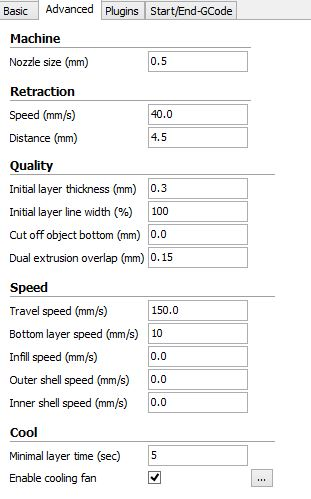
\includegraphics[scale=0.7]{res/CuraSettingAdvanced.JPG}
 \end{center}
\end{minipage}
\begin{minipage}{.47\textwidth}
Diese Einstellungen zu verändern ist meist nicht wirklich lohnenswert, allerdings manchmal hilfreich. Unter \textit{Machine} sollte man nichts verändern, da dies maschinenspezifisch ist. Diese Einstellung ist nicht druckrelevant, sondern abhängig vom Aufbau des Extruders. Unter dem Reiter \textit{Retraction} findet man die Einstellungen, wie weit das Filament bei Strecken, während denen nicht gedruckt wird, zurückgezogen wird, und wie weit der Extruder sich vom Druck abheben soll. Hier lohnen sich Veränderungen nicht.\\
Unter \textit{Quality} lassen sich von oben nach unten die Dicke der ersten Ebene, Linienabstand der Schicht, ob das Objekt unten abgeschnitten werden soll und (für den uns uninteressant, da nicht nutzbar) die Überlappung der Schichten bei zwei Extrudern einstellen.\\
\end{minipage}
\end{figure}
Unter \textit{Speed} lassen sich bestimmte Geschwindigkeiten einstellen. \textit{Travel speed} gilt für alle Strecken, bei denen nicht gedruckt wird (unter einer hohen Geschwindigkeit leidet die Qualität hier zwar nur wenig, allerdings spart man auch nicht viel Zeit), \textit{Bottom layer speed} nur für die unterste Ebene, welche für einen guten Druck eher langsam gedruckt werden sollte, \textit{Infill speed} gilt für Strecken, welche in Massivteilen gedruckt werden (bzw. in Rastern bei nicht voller Füllung), \textit{Outer} und \textit{Inner shell speed} gelten für die äußerste und innerste Schicht (Veränderung lohnt sich bei diesen dreien nur bei sehr großen Objekten mit viel Oberfläche oder Innenraum, der unsauber gedruckt werden kann oder sehr sauber gedruckt werden muss). \textit{0.0} als Wert heißt, dass die Standartgeschwindigkeit aus \textit{Basic} übernommen wird. \\
Unter \textit{Cool} findet man Einstellungen, welche die Kühlung betreffen. \textit{Minimal layer time} gibt die minimale Zeit einer Ebene an (sinnvoll bei sehr kleinen Objekten, damit die Ebene abkühlen kann, bevor die nächste darauf gedruckt wird; dies verhindert Unsauberkeiten). Unter \textit{Enable cooling fan} lässt sich der Kühler am Extruder einschalten, bei \textit{[...]} lassen sich außerdem weitere Einstellungen dazu finden. So kann man einstellen, ob der Lüfter erst ab einer bestimmten Höhe beginnt und/oder eine minimale oder maximale Geschwindigkeit hat. Bei einer Einstellung von 0.1 mm Schichtdicke und 0.2 für die erste Schicht, wird bei einer Einstellung von Gebläse ab 1mm ab der neunten Ebene der Lüfter aktiviert.
\subsection*{Druck starten}
\addcontentsline{toc}{subsection}{Druck starten}
Unter \textit{File} und \textit{Load model file} oder mit \textit{Strg} + \textit{L} lässt sich ein Mesh-, Bild-, oder GCodedokument öffnen. Das Objekt erscheint dann in der Mitte der Druckfläche und lässt sich dann mit der Maus verschieben oder nach einmaligem Klicken auf das Objekt in der unteren linken Ecke skalieren, drehen oder spiegeln. Außerdem kann man oben rechts verschiedene Ansichten wählen (u.a. Schichtweise wie oben, transparent oder mit markierten riskanten Überhängen).\\
Zusätzlich sieht man oben links, wie lange der Druck voraussichtlich dauert und wie viel Filament verbraucht wird (Länge und Gewicht). Nun kann man unter \textit{File}, \textit{Print...} oder \textit{Strg} + \textit{P} den Druck starten, nachdem das Objekt als GCode gespeichert wurde. Dafür muss der Drucker an den PC angeschlossen und ausgewählt sein (automatisch). Der Druck startet dann automatisch.\\
Alternativ lässt sich der Druck auch über die SD-Karte starten. Dafür muss im Druckermenü (am Gerät) die Karte gewählt werden und dann das Objekt mittels der Option \textit{Druck von SD-Karte} gedruckt werden. Dafür muss das Objekt vorher als GCode auf der Karte sein. Nachteil hierbei ist, dass es weniger Einstellungsmöglichkeiten gibt und diese zusätzlich noch schwieriger zu zu konfigurieren sind, weshalb wir den Druck mit PC und Kabel empfehlen. 
%---------------------------Niklas----------------------------------------------
\section{Probleme beim Drucken}
\iffalse
Probleme:
-Aus Extruder kommt nichts raus
-Druck hält nicht
-Extruder kratzt auf der Heizplatte
-Filament bricht
-Extruder verstopft (sollte bei Beachtung der anderen Fehler nicht passiere)
\fi

Beim Drucken von 3D Objekten können viele verschieden und unterschiedlich schwerwiegende Probleme auftreten. Hier sind diejenigen gelistet, die uns am häufigsten passiert sind:\\
\begin{description}

\item \textbf{Aus dem Extruder kommt nichts heraus.}\\
\addcontentsline{toc}{subsection}{Aus dem Extruder kommt nichts heraus}
Für dieses Problem kann es verschiedene Ursachen geben:
\begin{itemize}
\item \textit{Es ist kein Filament eingelegt:}\\
In diesem Fall ist der Extruder auf die für das gewünschte Filament benötigte Temperatur (PLA $210^\circ$C) zu erhitzen. Wenn dieser heiß ist, kann man das Filament in den Extruder einführen und den Extrudervorschub manuell erhöhen, bis unten Filament heraus tropft. Dies kann lange dauern, wenn der Extruder vorher leer war.\\
\textbf{ACHTUNG: Bei zu schnellem Vorschieben kann es passieren, dass das Filament sich nicht schnell genug erhitzt und dann den Extruder verstopft.}

\item \textit{Es ist vorher Filament aus dem Extruder gelaufen, ohne, dass welches nachgeschoben wurde:}\\
In diesem Fall muss der Extruder auf die für das gewünschte Filament benötigte Temperatur (PLA: $210^\circ$C) erhitzt werden. Wenn dieser heiß ist, kann man den Extrudervorschub manuell erhöhen, bis unten Filament unten heraus tropft. Dies kann lange dauern, wenn der Extruder vorher leer war.\\
\textbf{ACHTUNG: Bei zu schnellem Vorschieben kann es passieren, dass das Filament sich nicht schnell genug erhitzt und dann den Extruder verstopft.}
\end{itemize}

\item \textbf{Das gedruckte Objekt hält nicht auf der Heizplatte.}\\
\addcontentsline{toc}{subsection}{Das gedruckte Objekt hält nicht auf der Heizplatte}
Für dieses Problem gibt es keine ultimative Lösung. Wir haben haben mehrere Faktoren gefunden, die dafür verantwortlich sind:
\begin{itemize}
\item \textit{Temperatur der Heizplatte}\\
Die Temperatur der Heizplatte ist zumindest für PLA auf $60^\circ$ zu erhitzen.
\item \textit{Beschaffenheit des Objekts}\\
Je nach dem, ob das Objekt eine kleine Standfläche hat und hoch ist, bzw. eine sehr breite Standfläche hält es unterschiedlich gut. Weiterhin ist es wichtig einen \enquote{Brim} oder einen \enquote{Raft} zu drucken. Ein \enquote{Brim} sind mehrere Linien um das Objekt herum, die schnell zu drucken sind und den Halt der Objektes verbessern. Ein \enquote{Raft} hingegen ist eine Plattform, auf der das Objekt gedruckt wird. Diese hält durch eine besondere Beschaffenheit an der Unterseite besonders gut auf dem Heizbrett, dauert aber auch entsprechend lange zu drucken.
\item \textit{Position auf dem Heizbrett}\\
Wir haben festgestellt, dass Objekte die auf der linken, hinteren Ecke gedruckt werden besser halten als andere.
\item \textit{Der Extruder ist zu hoch über der Heizplatte}\\
Wenn der Extruder zu hoch über der Heizplatte druckt, kühlt das Filament ab, bevor es auf die Heizplatte trifft und hält dort nicht mehr. Daher sollte man \textbf{VORSICHTIG} den Extruder über die Knöpfe herunter fahren.
\item \textit{Wenn nichts hilft}\\
Sonst haben wir in einem Forum gelesen, dass Haarspray (möglichst das billigste) auf der Heizplatte den Halt stark verbessert. Momentan liegt ein Haarspray bei dem 3D-Drucker dabei und hat auch schon seine Dienste geleistet.
\end{itemize}

\item \textbf{Der Extruder kratzt auf der Heizplatte.}\\
\addcontentsline{toc}{subsection}{Der Extruder kratzt auf der Heizplatte}
Sollte der Extruder auf der Heizplatte kratzen, sollte der Druck direkt pausiert oder abgebrochen werden, um Schaden an der Heizplatte zu verhindern. Wenn auf der Heizplatte leichte schwarze Spuren zu erkennen sind, sollten diese im kalten Zustand der Heizplatte so weit wie möglich abgewischt werden. Das Problem liegt darin, dass die Heizplatte falsch gescannt wurde. Dies sollte dann nachgeholt werden. Auf dem 3D-Drucker im Menü \textit{Configuration/Z Calib./Heat Bed Scan} (siehe offizielles Manual S.57 ff.).\\
Temporär kann man dies auch über die manuelle Kontrolle des Extruders beheben, wobei man unbedingt aufpassen muss, dass der Extruder nicht die Platte zerstört oder die Platte den Z-Schalter.

\item \textbf{Das Filament bricht.}\\
\addcontentsline{toc}{subsection}{Das Filament bricht}
Wenn das Filament bricht ist es am sinnvollsten, das Filament direkt über dem Extruder, also zwischen Extruder und Z-Motor abzuschneiden und dann neues nachzufüllen. \textbf{ACHTUNG: dazu muss der Extruder auf die für das gewünschte Filament benötigte Temperatur (PLA: $210^\circ$C) erhitzt werden.} Danach sollte noch ein bisschen Filament nachgedrückt werden um zu gewährleisten, dass das neue Filament auch in den Extruder eingefüllt wird.

\item \textbf{Das Filament ist verknotet.}\\
\addcontentsline{toc}{subsection}{Das Filament ist verknotet}
Dies sollte möglichst vor dem Druck verhindert werden, da sonst das Filament während das Drucks bricht und der Druck damit nicht erfolgreich sein wird. Daher sollte das Filament auf der Rolle immer ordentlich aufgerollt sein und gegebenenfalls geordnet werden.

\item \textbf{Der Extrudervorschub dreht durch.}\\
\addcontentsline{toc}{subsection}{Der Extrudervorschub dreht durch}
Sobald der Extrudervorschub durchdreht gibt es genau zwei Möglichkeiten:
\begin{itemize}
\item \textit{Das Filament kann nicht in den Extruder eingeführt werden}\\
Wenn man gerade neues Filament eingeführt hat, kann es sein, dass das Filament an der Kante des Extruders hängen bleibt und daher nicht in den Extruder eingeführt werden kann. Dann sollte man vorsichtig mit einer dünnen Zange versuchen, das Filament in den Extruder zu leiten.
\item \textit{Der Extruder ist verstopft.}\\
Tja das ist sch****. Siehe unten.
\end{itemize}

\item \textbf{Der Extruder verstopft.}\\
\addcontentsline{toc}{subsection}{Der Extruder verstopft}
Jetzt weiß man auf jeden Fall, dass man einen der vorherigen Beschreibungen nicht richtig beachtet hat. Eigentlich ist der Extruder jetzt auszuwechseln, da dies aber kostspielig ist (\url{http://goo.gl/J6Bhq2} (Conrad.de 50\euro)) empfehlen wir zuerst zu versuchen, das Filament \textit{herauszuschmelzen}. Hierzu haben wir den Heizluftföhn der Schule verwendet und den oberen Teil des Extruders so lange erhitzt, bis das Filament auf raus gelaufen ist und keines mehr drin war. Hierbei muss man aber darauf achten, dass die Kabel nicht schmelzen bzw. der Extruder anderweitig beschädigt wird. Andere Leute haben in Foreneinträgen berichtet, dass Filament aus dem Extruder \textit{rausgebohrt} zu haben. Dies haben wir uns nicht getraut, da wir keinen Millimetergenauen Bohrer zur Hand hatten.

\item \textbf{Der Drucker wird nicht erkannt.}\\
\addcontentsline{toc}{subsection}{Der Drucker wird nicht erkannt}
Hierfür gibt es viele verschiedene Möglichkeiten:
\begin{itemize}
\item \textit{Der Drucker ist aus}\\
Hier sollte der Drucker an den Stromkreis des Hauses angeschlossen (am Besten an eine Steckdose) werden und daraufhin der Schalter auf der Rückseite des 3D-Druckers auf ein gestellt werden (I \textbf{nicht} O).
\item \textit{Das Kabel ist im PC oder im Drucker nicht eingesteckt}\\
Dies ist auch relativ einfach zu lösen. Hier sollte das Ende mit dem USB-Anschluss Type B in den Drucker eingesteckt werden und das Ende mit dem USB-Anschluss Type A in einen der USB Ports am PC.
\item \textit{Das USB-Kabel ist kaputt}\\
Nun sollte ein neues gekauft werden. Auf der einen Seite sollte dieses einen USB-Anschluss Type A (2.0 oder 3.0) haben und auf der anderen Seite einen USB-Anschluss Type B (2.0).
\item \textit{Der USB-Port ist kaputt}\\
Sollte der PC weitere USB-Ports besitzen, so sollten dieser als eine weitere Möglichkeit konsultiert werden, soweit dessen Version 2.0 oder höher ist.
\item \textit{Es sind keine Druckertreiber installiert}\\
In diesem Fall wurden die Treiber bei der Installation von Cura/RepetierHost nicht mit installiert. Das sinnvollste ist es diese Programme neu zu installieren und darauf zu achten, dass diesmal die Drucker Treiber installiert werden.
\end{itemize}
\end{description}
\end{document}